%% ---------------------------- OPERATING SYSTEM SPECIFICS ----------------------------
\section{Worker operating system configurations}
\label{s:WorkerOSConfiguration}
During the installation and initial setup of a worker, multiple configuration changes need to be applied in order to decrease the amount of noise traffic.
This noise traffic is primarily generated by the Ubuntu Linux packet managers APT and Snap, further elaborated in the section \ref{ss:DisableSnapAPT}.
Another noise generator is the network time protocol, described in section \ref{ss:DisableNTP}.
The use of these packet managers and an updated time through NTP is not relevant to use during this research and are therefore disabled.



%% ---------------- SNAP PACKET MANAGER ----------------
\subsection{Disabling automatic upgrades and stop package managers}
\label{ss:DisableSnapAPT}
Default delivered in Ubuntu Linux 20.04 is the older APT (Advanced Package Tool) and the newer Snap package manager. Packages delivered through the \textsc{Snap package manager} are called snaps.
There exist multiple methods of package management in Ubuntu, such as using Synaptic Package Manager, Ubuntu Software, apt, apt-get, or snap. It is also possible to download raw deb files and install them using the pkg tool. In the Ubuntu Software in Ubuntu 20.04, Snap is prioritized when installing packages in front of the commonly used APT package manager. DEB (Debian package format) packages are the older format for packages in Ubuntu Linux, which APT uses. Snaps are formatted differently and cannot be installed through APT but instead installed through the Snap package manager. The Snap package manager uses snapd daemon for package management. The Snap package format will replace the older DEB package in Ubuntu \autocite{petersen2020ubuntu}.

Noise traffic generated by the automatic update polling for the package managers can be reduced. A few configuration parameter changes must be implemented to disable the automatic updates.
Disabling automatic updates like this is a security risk for systems connected either to the internet or a local network. The workers are segmented on their own separated virtual network on one virtual host and not directly connected either to the internet or the local network. Therefore the risk during this research is acceptable.
By changing the given parameters for the auto upgrades seen in listing \ref{lst:AutoUpgradesApt} from $1$ to $0$ the automatic upgrades for the APT package manager are disabled.




\begin{listing}[!ht]
\caption{Disabling automatic updates for APT}
\label{lst:AutoUpgradesApt}
\begin{minted}{perl}
# File contents for /etc/apt/apt.conf.d/20auto-upgrades
APT::Periodic::Update-Package-Lists "0";
APT::Periodic::Unattended-Upgrade "0";
\end{minted}
\end{listing}
The snap package manager has a number of services running in Ubuntu 20.04 by default.
These services can be disabled by running two commands for each service.
The $systemctl$ $stop$ command stops the running service, while $systemctl$ $disable$ disables the service from running on startups. The commands in listing \ref{lst:DisableSnapServices} must be run as $root$ on the worker host in the Bash shell command prompt.
\begin{listing}[!ht]
\caption{Disabling Snap services}
\label{lst:DisableSnapServices}
\begin{minted}{Bash}
systemctl stop snapd
systemctl disable snapd
systemctl stop snapd.socket
systemctl disable snapd.socket
systemctl stop snapd.service
systemctl disable snapd.service
systemctl stop snapd.seeded
systemctl disable snapd.seeded
systemctl stop snapd.snap-repair.timer
systemctl disable snapd.snap-repair.timer
systemctl stop snapd.apparmor
systemctl disable snapd.apparmor
\end{minted}
\end{listing}

By implementing these changes the automatic updates will be disabled both for the APT package manager and the Snap package manager, and it will reduce the noise traffic generated.
%% ---------------- NTP ----------------
\subsection{Disabling NTP}
\label{ss:DisableNTP}
Default in a Ubuntu distribution, like the 20.04 used in this research, a time and date service is active for the purpose of keeping the system updated with the correct date and time.
The timedatectl would generate noise traffic such as NTP requests to ntp.ubuntu.com for synchronizing the time.
During the initial setup, before noise reduction measurements were taken, a significant number of NTP requests were sent from the worker in order to reach ntp.ubuntu.com.
The following command was executed to disable the network time
synchronization\footnote{\OrjansHref{https://www.man7.org/linux/man-pages/man1/timedatectl.1.html}{https://www.man7.org/linux/man-pages/man1/timedatectl.1.html}}.

\begin{listing}[!ht]
\caption{Command for disabling NTP synchronisation}
\label{lst:CommandDisableNTPSync}
\begin{minted}{Bash}
timedatectl set-ntp 0
\end{minted}
\end{listing}

This command stops the synchronisation services which enables the virtual machine to use the host's clock.
%% ---------------- TCPDUMP ----------------
\subsection{Enabling ordinary users to execute tcpdump}
\label{s:EnableTCPDumpNormalUsers}
tcpdump requires higher privileges to capture incoming and outgoing traffic on the network interface.
Since tcpdump is the program used for packet capturing in this research, it would be more efficient to give an ordinary user access to this program file and traffic capturing.
The design of the capture is that the scanner uses SSH to issue tasks to each worker host.
If tcpdump requires root access, this will lead to more complications in configurations on the worker host while issuing tasks to a worker.
This issue is mitigated by setting the set-user-ID bit on the tcpdump program, enabling unprivileged users to capture traffic on the worker host's network interface, which normally requires privileged access.

Since the worker hosts are located on an isolated virtual network, the risk of unauthorized access is reduced and enabling simplistic capture of packets without any advanced configuration changes.
These commands shown in listing \ref{lst:CmdChmodTcpdump} must be executed as $root$ on the worker to gain effect. The command in line one would return the full path for tcpdump, as seen in line two.
Line three changes the modifications on the program, setting the set-user-ID bit.
To assure that this is executed successfully, line four would list the permissions for the file shown inline five. Here we see that the $s$ flag is set for the owner ($-rws$) and the group ($r-s$), while a normal user has read and execution permissions ($r-x$).

\begin{listing}[!ht]
\caption{Command for changing mode on tcpdump file}
\label{lst:CmdChmodTcpdump}
\begin{minted}[linenos]{Bash}
which tcpdump
/usr/sbin/tcpdump
chmod +s /usr/sbin/tcpdump
ls -l /usr/sbin/tcpdump
-rwsr-sr-x 1 root root 1044232 Dec 31  2019 /usr/sbin/tcpdump
\end{minted}
\end{listing}

After setting the set-user-ID bit on the file, the file rights looks similar like mentioned in the listing above.

%% ---------------- /TCPDUMP ----------------
%% ---------------- NETWORK CONFIGURATION ----------------
\subsection{Network configuration}
\label{ss:WorkerNetworkConfiguration}
Within the setup of the lab environment, each worker host must have its unique network configuration.
For starters, a unique hostname needs to be set.
By executing the command as $root$ in listing \ref{lst:CommandHostnameCtl}, the hostname for the worker host is set.
\begin{listing}[!ht]
\caption{Command for setting hostname}
\label{lst:CommandHostnameCtl}
\begin{minted}{Bash}
hostnamectl set-hostname <hostname>
\end{minted}
\end{listing}

Within the research, the hostname convention used is $bscXY$, where the $XY$ symbolizes an incrementing number starting on \textit{01}.

Furthermore, the network configurations for each worker need to be set in the netplan configuration file shown in listing \ref{lst:NetworkCfg}. Within this file, both network interfaces are static configured. One NIC is used for the scanning traffic, and the second NIC is used for management traffic. To retrieve the name for each of the NICs's, the command $ip$ $a$ can be executed in the terminal. Result seen in listing \ref{lst:NetworkInterfaces}.

The IP subnet for the management network is chosen in accordance with RFC 1466 \autocite{rfc1466}.
The IP address block for the scanning network is chosen partly in accordance with RFC 5737 \autocite{rfc5737}, enlisted as $TEST-NET-1$ in the RFC and within this paper as \textsc{scanning network}. Different from the RFC standard is the subnet $192.0.2.0/24$ given in the RFC 5737 is not chosen since it's already used for another project within the local network.
To not create confusion, the $192.168.2.0/24$ subnet is chosen for this purpose, enlisted as \textsc{scanning network}.



\begin{listing}[!ht]
\caption{Network configuration for worker host}
\label{lst:NetworkCfg}
\begin{minted}[linenos]{yaml}
# File contents of /etc/netplan/00-installer-config.yaml
network:
  ethernets:
    ens33:
      addresses:
      - 192.168.2.110/24
      gateway4: 192.168.2.1
      nameservers:
        addresses:
        - 192.168.2.1
        search: []
    ens36:
      addresses:
      - 194.100.10.110/24
      gateway4: 194.100.10.1
      nameservers:
        addresses:
        - 194.100.10.1
        search: []
  version: 2
\end{minted}
\end{listing}

Within each of the netplan configuration files, a unique IP address needs to be set for each of the workers, as seen in listing \ref{lst:NetworkCfg}.
To reload the network configuration, execute $netplan$ $apply$ on the worker host as root.

These network settings can be verified after the settings are applied by running the command $ip$ $a$ on the worker host, resulting in a similar output as seen in listing \ref{lst:NetworkInterfaces}.
Within listing \ref{lst:NetworkInterfaces} we see that the scanning interface ($ens33$) have the IP address 192.168.2.110, which is validated against the configuration in listing \ref{lst:NetworkCfg}, while the management network is set to $ens36$ with the IP address 194.100.10.110.


\begin{listing}[!ht]
\caption{Listing of network interfaces}
\label{lst:NetworkInterfaces}
\begin{minted}[fontsize=\footnotesize]{Bash}
1: lo: <LOOPBACK,UP,LOWER_UP> mtu 65536 qdisc noqueue state UNKNOWN group default qlen 1000
    link/loopback 00:00:00:00:00:00 brd 00:00:00:00:00:00
    inet 127.0.0.1/8 scope host lo
       valid_lft forever preferred_lft forever
2: ens33: <BROADCAST,MULTICAST,UP,LOWER_UP> mtu 1500 qdisc fq_codel state UP group default qlen 1000
    link/ether 00:11:22:33:44:55 brd ff:ff:ff:ff:ff:ff
    inet 192.168.2.110/24 brd 192.168.2.255 scope global ens33
       valid_lft forever preferred_lft forever
3: ens36: <BROADCAST,MULTICAST,UP,LOWER_UP> mtu 1500 qdisc fq_codel state UP group default qlen 1000
    link/ether 00:22:33:aa:ff:44 brd ff:ff:ff:ff:ff:ff
    inet 194.100.10.110/24 brd 194.100.10.255 scope global ens36
       valid_lft forever preferred_lft forever
\end{minted}
\end{listing}

In Linux, there is a file located in $/etc/hosts$, shown in listing \ref{lst:EtcHostsScannerHost}, which is a local DNS file for looking up locally defined DNS records.
On the scanning host for this research, this file contains the IP addresses of each of the workers IP addresses.
The file has entries for both network interfaces, scanning network, and management network as described in section \ref{ss:WorkerNetworkConfiguration}.

\begin{listing}[!ht]
\caption{Contents of /etc/hosts on scanner host}
\label{lst:EtcHostsScannerHost}
\begin{minted}[fontsize=\footnotesize]{Bash}
127.0.0.1       localhost
127.0.1.1       kali
192.168.2.101   bsc01
192.168.2.102   bsc02
192.168.2.103   bsc03
192.168.2.104   bsc04
192.168.2.105   bsc05
192.168.2.106   bsc06
192.168.2.107   bsc07
192.168.2.108   bsc08
192.168.2.109   bsc09
192.168.2.110   bsc10
192.168.2.111   bsc11
192.168.2.112   bsc12
192.168.2.113   bsc13
192.168.2.114   bsc14
192.168.2.115   bsc15
192.168.2.116   bsc16
192.168.2.117   bsc17
192.168.2.118   bsc18
192.168.2.119   bsc19
192.168.2.120   bsc20
194.100.10.101   bsc01-mng
194.100.10.102   bsc02-mng
194.100.10.103   bsc03-mng
194.100.10.104   bsc04-mng
194.100.10.105   bsc05-mng
194.100.10.106   bsc06-mng
194.100.10.107   bsc07-mng
194.100.10.108   bsc08-mng
194.100.10.109   bsc09-mng
194.100.10.110   bsc10-mng
194.100.10.111   bsc11-mng
194.100.10.112   bsc12-mng
194.100.10.113   bsc13-mng
194.100.10.114   bsc14-mng
194.100.10.115   bsc15-mng
194.100.10.116   bsc16-mng
194.100.10.117   bsc17-mng
194.100.10.118   bsc18-mng
194.100.10.119   bsc19-mng
194.100.10.120   bsc20-mng
\end{minted}
\end{listing}




%% ---------------- SSHD CONFIGURATION ----------------
\subsection{SSH configurations}
\label{ss:SSHConfiguration}
By default the SSH service are listening on $0.0.0.0$, meaning all interfaces, as seen in the red marked two lines in figure \ref{fig:SSHMngNetwork}.
To achieve the objective regarding minimizing noise traffic to the scanning network interface, the SSH service used for task management must be set to listen to the correct network interface. The usage of SSH on the scanning network interface are not relevant and are therefore strictly limited to the management interface.
The listen address parameter in the SSHd configuration file needs to be changed to the IP address for the management network interface, as seen in listing \ref{lst:SSHDConfiguration}. This parameter change is conducted on each worker through opening the virtual machine in VMware Workstation. The $root$ user must conduct this, since the SSHd configuration file is a file owned by root.
The IP address in line number 2 in listing \ref{lst:SSHDConfiguration} must be changed accordingly to the IP address assigned to the management network interface on the given worker host.

\begin{listing}[!ht]
\caption{Limiting SSH to listen only to the management NIC}
\label{lst:SSHDConfiguration}
\begin{minted}[linenos]{apacheconf}
# Changed parameters from default in file /etc/ssh/sshd_config
ListenAddress 194.100.10.110
\end{minted}
\end{listing}

After this change is done, the SSH service must be restarted.
This must be done by elevating the privileges to $root$ and execute the command in listing \ref{lst:RestartSSHserver}.

\begin{listing}[!ht]
\caption{Restart SSH server}
\label{lst:RestartSSHserver}
\begin{minted}{Bash}
systemctl restart ssh
\end{minted}
\end{listing}

After the SSH server are restarted, the listen address must be validated.
This could be done by executing the command in listing \ref{lst:VerifySSHListening}, and the result of this command is shown in figure \ref{fig:SSHMngNetwork}.
\begin{listing}[!ht]
\caption{List of listening services}
\label{lst:VerifySSHListening}
\begin{minted}{Bash}
ss -lntu
\end{minted}
\end{listing}

\begin{figure}[htbp]
\centerline{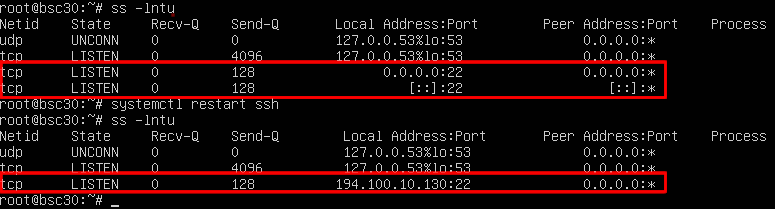
\includegraphics[scale=0.55]{images/misc/SSH-Verified.png}}
\caption{Verifying SSH configuration ListenAddress for management network.}
\label{fig:SSHMngNetwork}
\end{figure}

The last red marked line in figure \ref{fig:SSHMngNetwork} shows that the server only listens to incoming traffic on port 22 when the address is $194.100.10.130$. This means the SSH listening address is verified to only accept incoming connections on the mentioned address.


Furthermore, the key exchange between scanner and worker must be configured.
As a first-time procedure, the key generation for the scanner host needs to be conducted in order to achieve automatic login to a worker without a password prompt.
The command in listing \ref{lst:SSHKeyGeneration} is executed on the scanner host to generate a key pair with both private and public keys.


\begin{listing}[!ht]
\caption{SSH key generation}
\label{lst:SSHKeyGeneration}
\begin{minted}{Bash}
ssh-keygen -t rsa
\end{minted}
\end{listing}


When the key pair is generated, a simple SSH client configuration needs to be implemented in order to achieve automatic login through SSH without receiving a password prompt.
This configuration checks if the worker's hostname matches the criteria $bsc*-mng$, shown in line 2 in listing \ref{lst:SSHClientConfiguration}. In case of a match of the criteria, the configuration defines which default usernames are used to successfully connect to the worker host, shown in line 3 in listing \ref{lst:SSHClientConfiguration}. Also, the given private key to use for the connection is defined in line 4 in listing \ref{lst:SSHClientConfiguration}.

The configuration in listing \ref{lst:SSHClientConfiguration} must be implemented to the file referred to in line 1 on the scanner host to achieve this.

\begin{listing}[!ht]
\caption{SSH client configuration for scanner host}
\label{lst:SSHClientConfiguration}
\begin{minted}[linenos]{apacheconf}
# Implement the following lines to the file /root/.ssh/config
Host bsc*-mng
    User bscadm
    IdentityFile ~/.ssh/id_rsa
\end{minted}
\end{listing}

When these settings are implemented, the public key needs to be authorized on the worker host.
This is step two of the process of enabling authorization using a public key instead of a password prompt.
\begin{listing}[!ht]
\caption{SSH key authorization on worker host}
\label{lst:SSHKeyAuthorization}
\begin{minted}[linenos]{Bash}
ssh-copy-id -i ~/.ssh/id_rsa bscadm@bsc30-mng
ssh bsc30-mng
\end{minted}
\end{listing}

The command in line 1 in listing \ref{lst:SSHKeyAuthorization} adds the key to the authorized keys list in the home directory for the user $bscadm$, as defined in line 3 in listing \ref{lst:SSHClientConfiguration}.
Secondly, in line 2 in listing \ref{lst:SSHKeyAuthorization}, the connection is tested.
The first time logging in on this worker would trigger a prompt for key authorization, which must be accepted before continuing.
From this point forward, the ability to automatically log in to a worker using public-key authorization is enabled.



%% ---------------- /SSHD CONFIGURATION ----------------
%------ LAB ENVIRONMENT ------
\subsection{Lab environment}

Through an initiation worker preparation script, there are implemented commands to reduce traffic noise affecting the scan results. This script disables certain services known for querying servers on the internet for the purpose of updating time through NTP, automatic operating system updates, and operating system package updates. This script must be run during the setup of the environment to ensure noise reduction. Another very important step during this initial configuration is change moving the tcpdump command to suid ($chmod +s$), meaning a regular user is able to run tcpdump as a regular user. The command must be executed by root. During the initial configuration of each worker, the SSH public key for the scanner host is added to the worker's authorized keys in $\$HOME/.ssh/authorized\_keys$. It allows the scanner host to remotely access each worker with the use of its SSH private key to manage tasks for the worker through SSH. Each worker has its own $bscadm$ local user for this purpose. SSH listens only to the management network interface on each worker.